\chapter{The optimization of Collective Actions by Individual Selection}
\label{chapter:C1_article2}

\setcounter{secnumdepth}{0}
\setcounter{minitocdepth}{1}
\minitoc[n] % minitoc without title

In this Chapter, we investigate how the nature of coordination behaviours influences the optimization of collective actions. This Chapter is presented as a draft for a journal article.

In the previous Chapter we revealed that the evolution of collective actions was hindered by the evolution of coordination. In particular, we used evolutionary robotics to shed a light on the mechanistic constraints at play in the transition from a solitary to a cooperative equilibrium. Here we are interested in understanding how individual selection can lead to the transition between different collective equilibria.

Collective actions reap their benefits through the interactions between multiple individuals. However while they may benefit every individual in a mutualistic fashion, it is not clear how these collective behaviours are reached. More precisely, because they require the coordination of several individuals, multiple stable equilibria can emerge. Additionally, because benefits are reached through a collective action, a single individual deviating from the evolved equilibrium would not be favored by selection. In other words, a mutant acting toward a different collective equilibrium would not be selected, even if the equilibrium is more advantageous for the group. In consequence, the issue of the optimization of collective actions arises. Namely we wonder how it is possible for individual selection to lead the transition toward an optimal equilibrium when another collective equilibrium already evolved ?

One classical mechanism to solve this issue is group selection. Because those behaviours are beneficial at the level of the group then selection could only occur at the same level, so the argument goes. Here we study if collective behaviours could be optimized by individual selection only. To that end, we model the example of collective hunting. Individuals evolve in an environment where they can hunt two differently rewarding types of prey: \emph{boar} and \emph{stag}. Each type of prey corresponds to a different collective equilibrium: suboptimal for the boar and optimal for the stag. Our goal is thus to study the transition from the suboptimal equilibrium (i.e. boar hunting) to the optimal equilibrium (i.e. stag hunting).

We reveal that under simple ecological features where only two prey are present in the environment, the transition to the optimum is impossible. However, under more realistic assumptions where the individuals have to choose between multiple prey, then the optimal equilibrium evolved in $8$ replications out of $30$. In particular, the individuals now have to coordinate in order to achieve cooperation. This means that they need to react to each other's behaviour. From this it stems that they also react to a mutant's behaviour. This in turn may allow the group to reap the benefits of stag hunting. 

However, in the collective strategy evolved by the individuals, they both separately decide which prey to hunt, leading to weak coordination. We then study how a more asymmetrical coordination strategy could impact the transition to the optimum. To that end, we increase the complexity of the neural networks controlling the individuals in order to allow them to evolve more complex coordination strategies. In this case, we reveal that the transition to the optimum is facilitated as stag hunting evolves in $24$ replications out of $30$. Furthermore, we observe the evolution of a more efficient asymmetrical strategy where the individuals adopt two different roles: the \emph{leader/follower} strategy. In this strategy, only the leader decides on which prey to hunt and the follower goes on the same prey. In consequence, while choosing to cooperatively hunt a stag was previously a collective decision making problem, it is now an individual problem. This means that a mutant leader going for a stag is now sufficient for both individuals to reap the benefits of stag hunting. Moreover, the leader/follower strategy evolved because it was more efficient for each individual. Thus we show that the evolution of an individually adaptive coordination strategy may lead to the optimization of a collective behaviour.

\clearpage

\begin{flushleft}
\textbf{\Huge The Optimization of Collective Actions by Individual Selection}
\end{flushleft}

\section{Abstract}
  Many social behaviours lead to the coexistence of multiple stable equilibria. However, a single individual deviating from a given collective equilibrium can not be favored by selection. In consequence the selection of the optimal equilibrium when another collective equilibrium already emerged is commonly explained by group selection. Here we study the optimization of group traits thanks to individual selection alone. We focus on a problem of collective hunting, where individuals have to choose between a suboptimal and an optimal prey, which we model in evolutionary robotics. We reveal that while the switch to the optimum is impossible under unrealistic environmental conditions, it can occur when the environment is more complex. In particular, when coordination is necessary to cooperate, individuals react to each other's behaviour. As such a mutant's behaviour can affect that of the group and lead to the optimum. We then reveal that when a more efficient coordination strategy is evolved, the transition to the optimum is highly facilitated. Furthermore, the evolution of this new strategy is individually beneficial and was not enforced on the individuals. In consequence, we show that  the optimization of collective action can occur by individual selection.


\section{Introduction}
  Many social traits are beneficial thanks to the emergence of collective features. For instance, collective hunting may allow to kill stronger or faster prey than what could be done in a solitary fashion. However this behaviour is only individually adaptive in interaction with a group of other collective hunters. The benefits of these behaviours are thus reached through the emergence of a group-trait. This raises the issue of how they could evolve under individual selection.

  Once a collective strategy has emerged, a single mutant following a different strategy would not be favoured by selection. As such multiple evolutionarily stable equilibria may exist, as is the case in coordination games~\parencite{MaynardSmith1982a, Skyrms2004}. Yet it is not clear how to predict which equilibrium will emerge. In particular, individuals may evolve a suboptimal equilibrium instead of the optimal one. Therefore, because no individual can benefit by deviating from the equilibrium evolved by the group, this raises the issue of optimizing the collective behaviour. Namely, how can the optimal equilibrium be reached when a suboptimal equilibrium has already emerged ?

  A popular mechanism to explain the selection of equilibria is that of group selection~\parencite{Boyd1990}. Because these collective traits are adaptive at the level of the group it seems that only a selective pressure acting at the same level can lead to their optimization. Different groups will reach various collective equilibria and thus benefit differently from the evolved equilibria. In consequence, the groups for which a higher payoff equilibrium emerged will be at a selective advantage in comparison to others and their strategy is thus expected to spread in the population. The evolution of cultural norm in particular is a popular group-level explanation for the emergence of collective traits in Humans~\parencite{Boyd2002, Binmore2011, Smaldino2014}.

  In this article, we show that the optimization of collective actions can be reached thanks to individual selection alone. To that end, we take the example of collective hunting. Because it is necessary to agree on which prey to hunt, this behaviour requires the coordination of several individuals~\parencite{Alvard2002, Alvard2003, Drea2009a}. This implies that a single mutant choosing a different prey than that agreed upon would not benefit from this behaviour. Thus several equilibria can evolve. The group can specialize on the optimal prey, but it can also specialize on suboptimal ones. In this case no individual mutation can divert the group from a suboptimal prey. Here, we want to understand how individual selection can switch the group's strategy towards the optimal prey.

  To that end, we model collective hunting in evolutionary robotics~\parencite{Nolfi2000, Doncieux2015a}. We use evolutionary robotics in this context as it allows to study the nature of the coordination behaviours evolved which, we will show, turn out to have critical effects on collective optimization. Evolutionary robotics has been previously applied to model the mechanistic constraints at play in the mapping between genotype and phenotype~\parencite{Mitri2013, Trianni2014b, Bernard2016a}. We design a setting where a pair of individuals can hunt two different types of prey: a suboptimal one and an optimal one. For the sake of simplicity (and not behavioural realism) we choose to arbitrarily call these two prey respectively boar and stag. The reward from hunting a prey depends on the type of prey hunted and the manner in which it is hunted: solitarily or cooperatively. More precisely, two robotic agents are placed in an arena where they can capture non-moving prey. Both these agents are controlled by artificial neural networks, whose connection weights are evolved (see \emph{Materials and Methods} for further description of the experimental setting). resulting from the evolved genotypes. Thus, individuals have to coordinate in order to hunt in a cooperative manner. We design the model so that the individuals have evolved the suboptimal equilibrium and that it is not beneficial for a single individual to switch to a different prey alone. We study under which conditions could the transition to the optimal equilibrium occur.

  We show that the transition from the suboptimal to the optimal equilibrium is impossible under simple environmental conditions. However, in a more realistic setting, individuals are expected to be able to coordinate. We reveal that when this is the case, the evolution of coordination also enables the switch toward the optimum. Furthermore, the nature of coordination strategies also happens to change the probability for this switch to occur.


\section{Materials and Methods}
\label{sec:matandmet}
  \subsection{Experimental Setup}
    The environment is constituted of a $800$ by $800$ units arena with four solid walls. We place a collection of circular agents (with a diameter of $20$ units) in this arena. The agents are divided between two categories: predators and prey. Predators can move freely in the environment according to the inputs of their sensors which are comprised of several proximity sensors and a camera. Proximity sensors are evenly distributed around the robotic agent's body and have a range of twice the body's diameter. Each of these proximity sensors gives the agent the distance to any obstacle (walls or other agents) it senses in its direction. In comparison, the camera is placed on the front of the robotic agent and is constituted of $12$ rays spread in a $90$ degrees cone. Each ray gives the type (hunter, boar or stag) and proximity of the nearest agent in its direction. Each hunter begins the simulation next to the other agent at one side of the arena.

    In opposition to the predators, prey are static and stay at their initial position until either the end of the simulation or their capture by a hunter (experiments with moving prey capable of avoidance behaviours did not show significantly different results). For a prey to be successfully captured, a hunter needs to remain in contact of this prey for $800$ time steps (out of a total number of $20000$ simulation steps). The hunter is then rewarded with the value corresponding to the prey. The prey is finally removed from the environment and replaced at a random position in the arena. We thus ensure that both the number of prey and the ratio of the types of prey are kept constant. We consider that collective hunting happens when both hunters are in contact of the prey at the last time step of its capture. This implies that is not necessary for the two agents to be in contact of the prey during all of the hunting time for cooperation to happen.

    Each hunter is controlled by a fully-connected multilayer perceptron with a single hidden layer. The inputs of this neural network are constituted of all the sensory information of the agent and a bias neuron whose value is always $1$. $1$ input neuron is used for each of the $12$ proximity sensors and $3$ neurons for each of the $12$ rays of the camera (the type of an agent is encoded by $2$ binary values and $1$ value is used to encode proximity). In consequence, the total number of input neurons amounts to $49$. The hidden layer is constituted of $8$ neurons while the output layer has $2$ neurons, each one of them encoding for the speed of each of the agent's wheels. While the connection weights of the network are evolved, the topology is kept identical. Finally, the mapping function used to compute the outputs is a sigmoid.


  \subsection{Simulating Artificial Evolution}
    The genome has a varying size. Indeed, to increase neural complexity, each individual can evolve two topologically similar neural networks. At the start of evolution, genomes are initialized with $410$ real values sampled uniformly in the range \([0,1]\). This amounts to the number of connection weights of a single neural network. At each generation of the algorithm, a genome encoding for a single neural network has a probability of \(5 \times 10^{-2}\) to be duplicated. When a duplication event occurs, the genome then encodes separately for the two neural networks, which means that its size is $820$. Each generation, there is also a probability of \(5 \times 10^{-3}\) that a deletion event occurs for a genome which encodes for two neural networks. If this happens, one of the two neural networks encoded by this genome is randomly lost and the size of this genome is reverted back to $410$.

    Evolution is simulated by a classical evolutionary algorithm. At each generation of the algorithm, every individual is paired $5$ times with a randomly chosen partner (which may be different each time). Each of these pairs is then independently evaluated in the environment during $20000$ steps. In order to decrease the stochasticity effects occuring because of the random positioning of the prey, each pair is evaluated $5$ times. Hence $25$ simulations are performed for each individual per generation. The fitness of an individual is then computed as the average reward obtained over these $25$ simulations.

    Selection is conducted according to a \((10 + 10)\) elitist selection strategy. Namely, the population of the next generation is constituted of the $10$ best individuals of the previous generation and $10$ offsprings sampled from these $10$ best individuals. Each offspring is a mutated clone of its parent and no recombination is used. Mutations are sampled according to a Gaussian operator, with a standard deviation of \(2 \times 10^{-1}\) and a per-gene mutation probability of \(5 \times 10^{-3}\). Finally, each experiment was conducted during $9000$ generations and replicated $30$ times.

\section{Results}
  \subsection{The transition to the optimum is impossible}
    In this first experiment, we are interested in the transition to the optimum strategy in a very simple environment w.r.t. collective hunting. More precisely, individuals are evolved in an environment constituted of only a single prey of each type. Rewards for hunting are summarized in Table~\ref{table:tableRewards}. The agents are initially pre-evolved during $3000$ generations in an environment where hunting stags grants nothing. We thus ensure that the suboptimal equilibrium (i.e. hunting boars cooperatively) has been evolved. Then the individuals are evolved during $6000$ additional generations where hunting stags is rewarded.

    \begin{table}[ht]
      \centering
        \begin{tabular}{|l|r|c|}
          \hline
          \multicolumn{2}{|l|}{\textbf{Prey}} & \textbf{Food Reward} \\
          \hline
          \hline
          \textbf{Boar} & \textit{alone} & 50 \\
          \hline
          & \textit{coop.} & 125 \\
          \hline
          \textbf{Stag} & \textit{alone} & 0 \\
          \hline
          & \textit{coop.} & 250 \\
          \hline
        \end{tabular}
        \caption{\textbf{Food Rewards for hunting.}
        Rewards depend on whether the hunt was solitary or cooperative.}
      \label{table:tableRewards}
    \end{table}

    We show in Figure~\ref{fig:figControl}(A) the mean proportion of each type of prey hunted over evolutionary time in $30$ independant replicates. Figure~\ref{fig:figControl}(B) shows the proportion of prey hunted at the last generation of evolution in each replicate. We observe that during the pre-evolution step, a cooperative strategy was evolved on the boars. However even after this step, there was no transition towards hunting stags. This implies that is in this case the switch from the suboptimal equilibrium to the optimal equilibrium is impossible. 

    %In particular, while cooperation was evolved during the pre-evolution step, no coordination strategy was necessary to cooperate under such ecological conditions. Because there is only one prey of each type, there is no need to react to the other individual in order to collectively decide on which prey to choose.

    \begin{figure}[h]
      \centering
        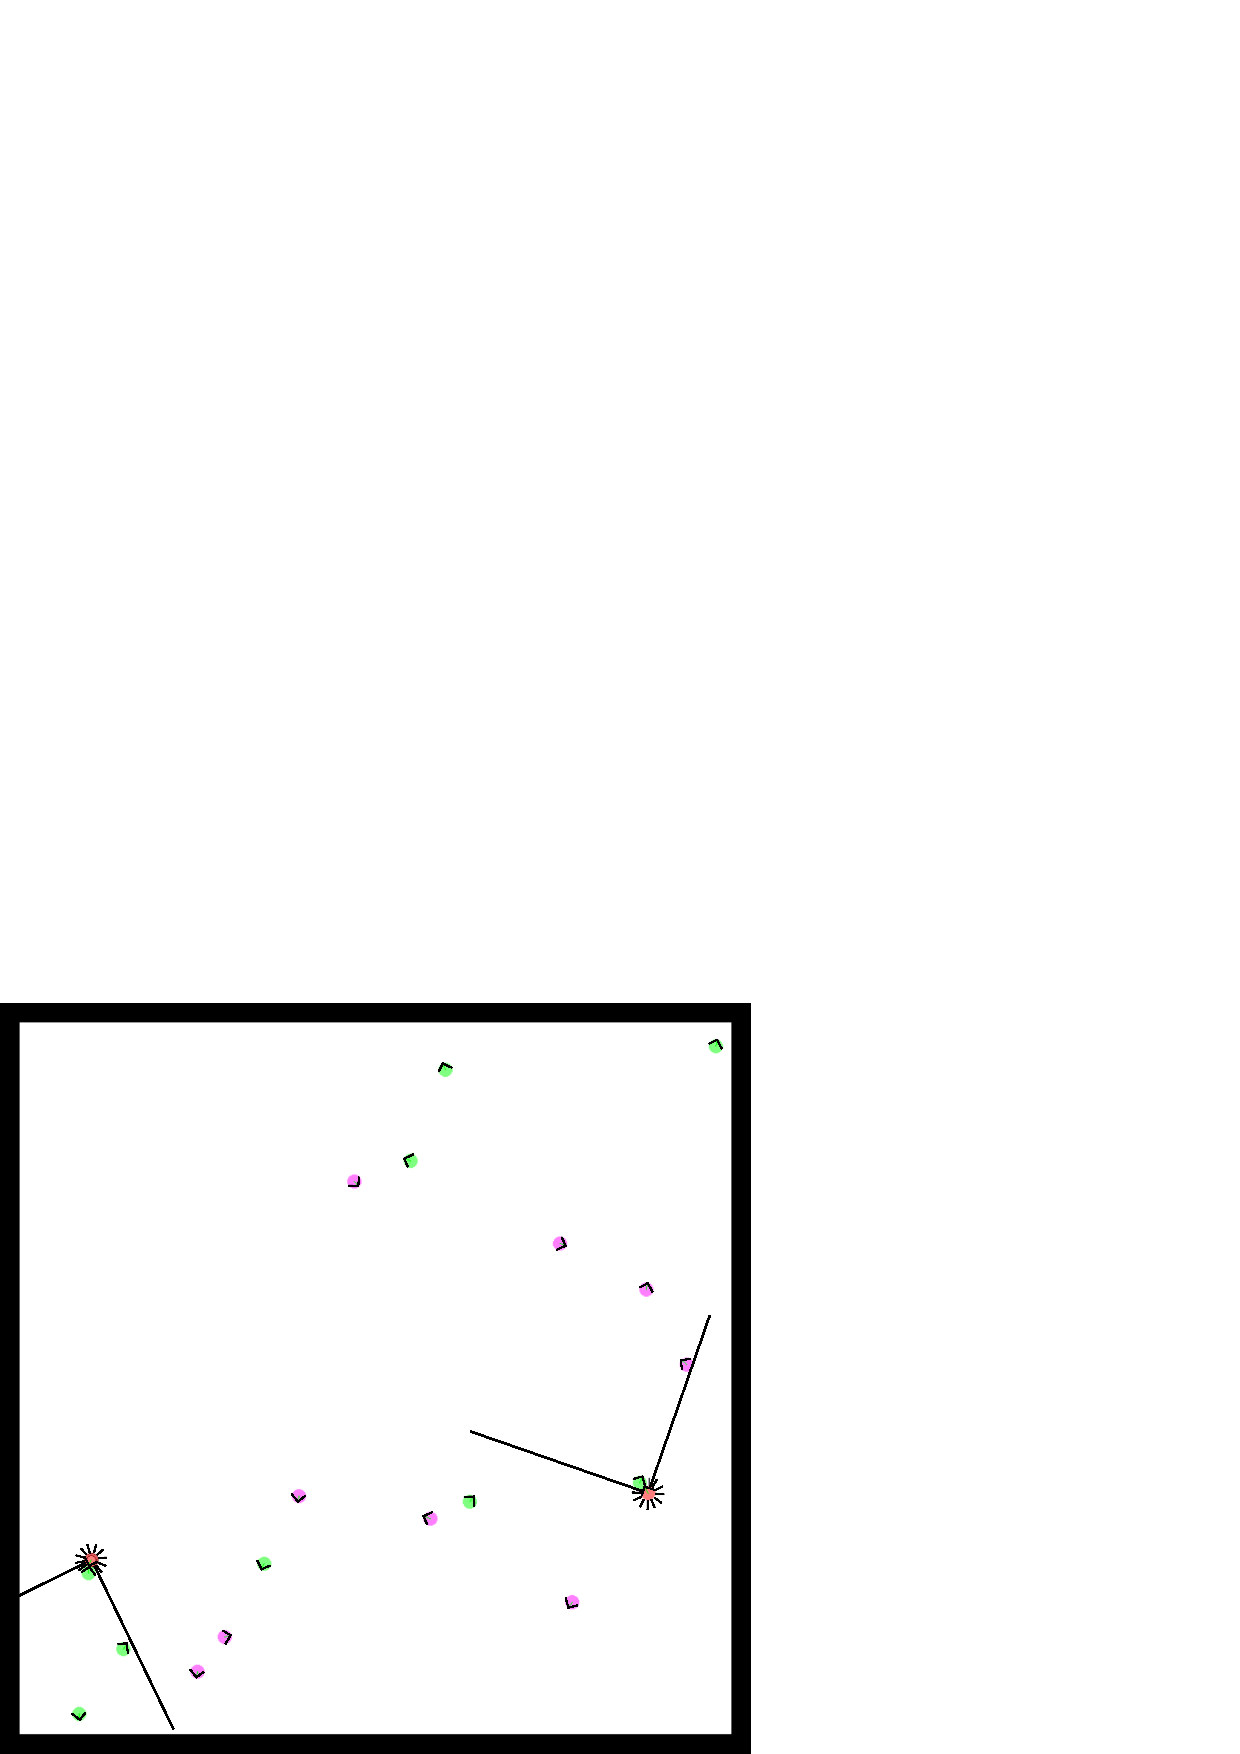
\includegraphics[width=1\linewidth]{fig/ArticleBio2/Fig1.png}
        \caption{\textbf{Mean proportion of prey hunted cooperatively.}
        \emph{(A)} Mean proportion of boars and stags hunted cooperatively by the best individual in each of the $30$ independant replications. The colored areas around the medians represent the first and third quartiles. The red line represents the separation between the pre-evolution step (when hunting stags rewards nothing) and the rest of the evolution. \emph{(B)} Repartition of the prey hunted at the last generation of evolution by the best individual in each replication. Rewards for a boar are 50 if hunted alone and 125 if hunted cooperatively. A stag hunted alone rewards 0 and 250 if hunted in a cooperative fashion (Table~\ref{table:tableRewards}).}
      \label{fig:figControl}
    \end{figure}

  \subsection{The optimum can be reached under more realistic environmental features}
    However, it is unrealistic to consider collective hunting only under such extreme ecologicial conditions. In particular, in nature hunters are expected to collectively choose which prey to hunt from multiple similar prey. To that end, individuals are now evolved in an environment constituted of $18$ prey, half of them being boars, the other half being stags. As previously, individuals are first pre-evolved during $3000$ generations in an environment where stags do not provide any reward. We then want to study the impact of these new environmental conditions on the transition to the collective optimum (i.e stag hunting).

    We show in Figure~\ref{fig:figRecycling}(A) the number of replicates out of $30$ where the optimal equilibrium evolved. More precisely, we consider that this equilibrium was achieved when more than \(50\%\) of the prey hunted were stags hunted cooperatively. We present the results from two different settings: the \emph{Control} setting and the \emph{Coordination} setting. The Control setting corresponds to what was presented in the previous Section, where the environment is only constituted of one boar and one stag, to act as comparison with the new results. The Coordination setting corresponds to the setting presented in the last paragraph (i.e. $18$ prey in the environment). We observe that the evolution of cooperation on the stags is facilitated as it evolves in $8$ replicates out of $30$. 

    \begin{figure}[h]
      \centering
        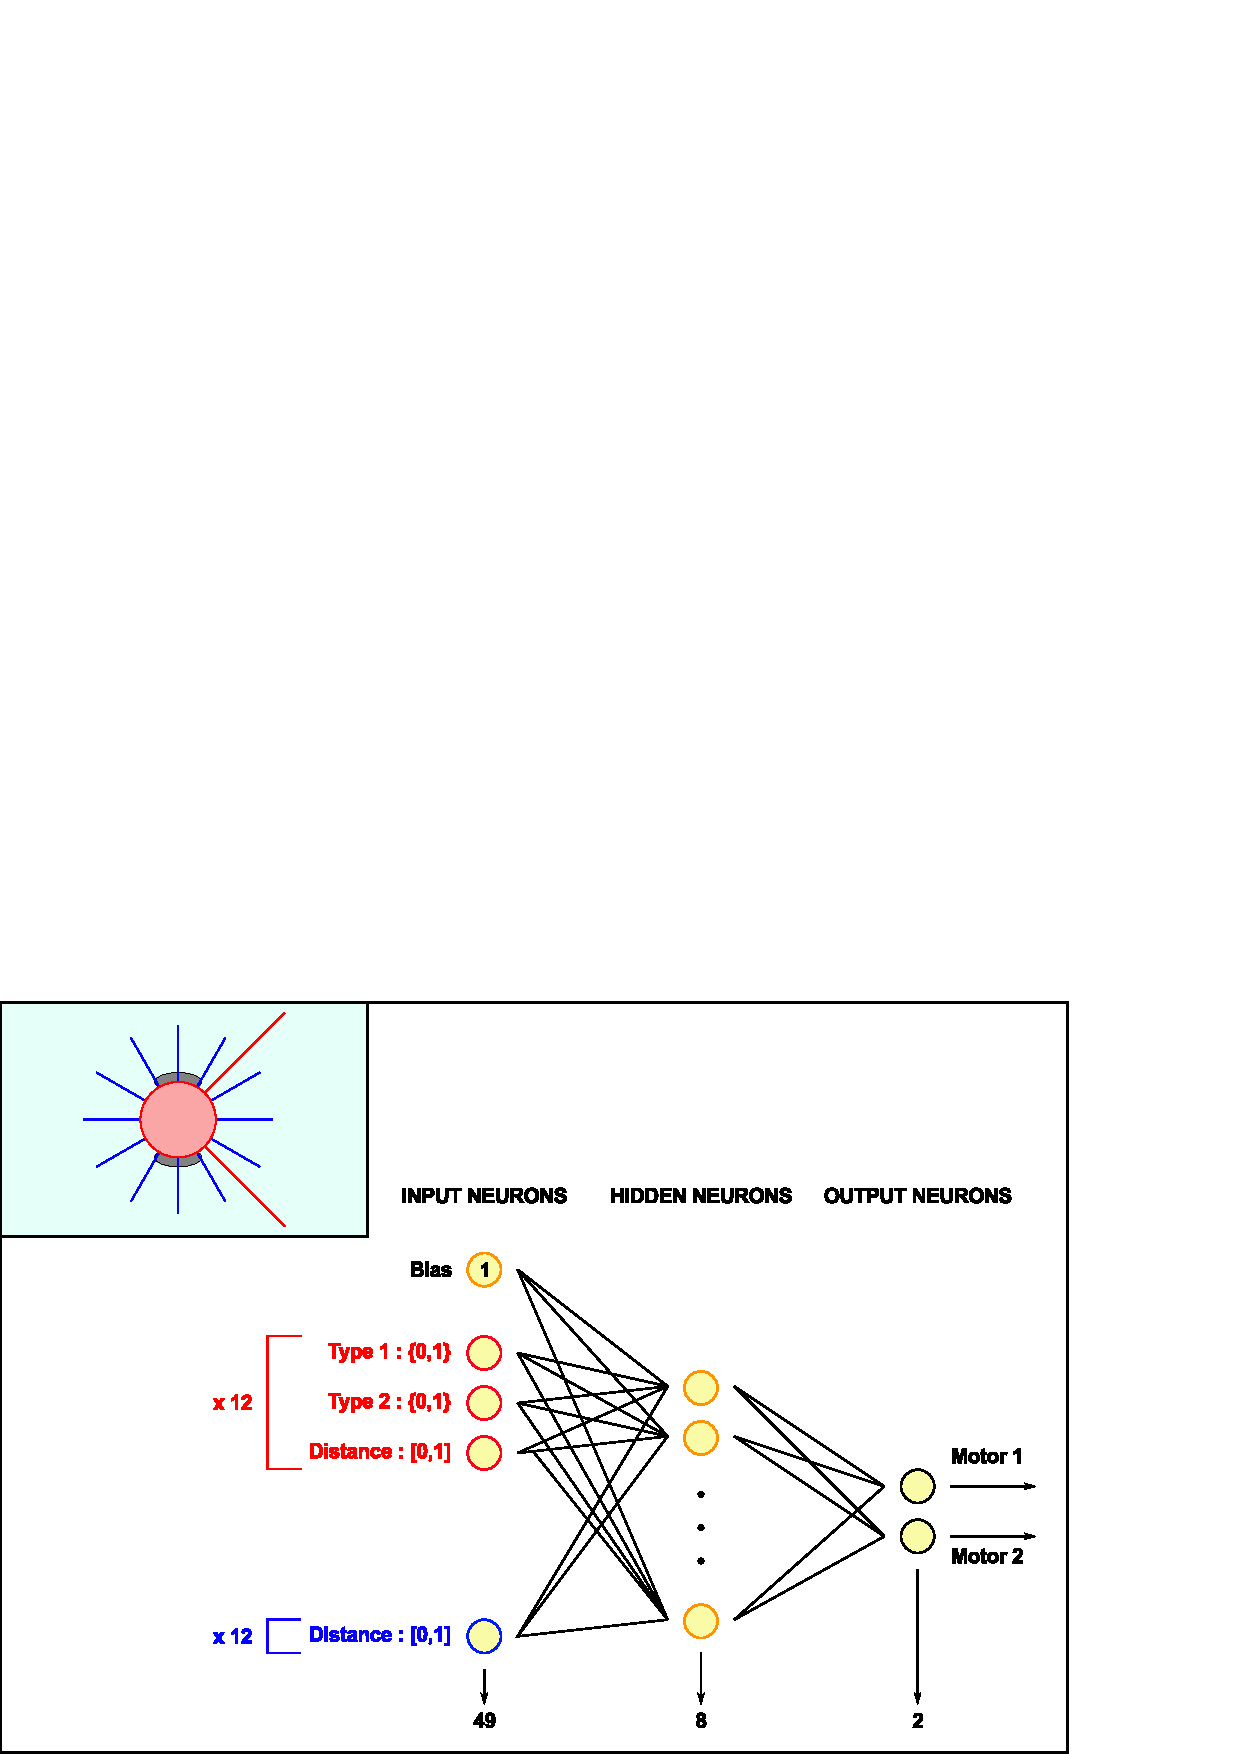
\includegraphics[width=1\linewidth]{fig/ArticleBio2/Fig2.png}
        \caption{\textbf{Proportion of stag hunting runs and proportion of prey hunted.}
        \emph{(A)} Number of replications (out of a total of $30$) where stag hunting evolved in the \emph{Control} and \emph{Coordination} settings. We consider that stag hunting evolved when more than $50\%$ of the prey hunted were stags hunted cooperatively. In the Control setting, the environment is constituted of one boar and one stag. In comparison, in the Coordination setting, $18$ prey are present in the environment and it is thus necessary to coordinate for cooperation to happen. Rewards for a boar are 50 if hunted alone and 125 if hunted cooperatively. A stag hunted alone rewards 0 and 250 if hunted in a cooperative fashion (Table~\ref{table:tableRewards}). \emph{(B)} Repartition of prey hunted at the last generation of evolution by the best individual in every replications in the Coordination setting. The population for each of the replications was previously evolved in an environment where hunting stags rewards nothing.}
      \label{fig:figRecycling}
    \end{figure}

    A striking difference with the previous experiment is that, because of more complex environmental conditions, individuals now evolve a coordination strategy. This behaviour, which we call the \emph{turning} strategy, is shown in Figure~\ref{fig:figTurningBehaviour}. When individuals adopt this behaviour, they constantly turn around one another. This way, they ensure that they keep the other individual in their line of sight. At the same time, they move towards a prey and, thanks to their proximity, when one of them gets on a prey the other can join it quickly. In consequence, they are able to achieve cooperation to solve the issue raised by the necessity to decide on which prey to hunt (Figure~\ref{fig:figRecycling}(B)). More importantly, because the hunters now react to each other, the behaviour of a mutant can affect that of the other individual. This explains why the transition to the optimal equilibrium was enabled.

    However we can observe several drawbacks from this strategy. All these drawbacks come from the fact that both individuals adopt a symmetrical behaviour. In particular, they both steer towards a desired prey and thus react only weakly to the other individual's behaviour. First, as both individuals can guide the group towards a different prey, this may lead to a situation where it is hard to achieve consensus between them. This can considerably slow them down and thus cause suboptimal performance w.r.t. the number of prey hunted. Then, if prey are close to one another, the fact that both individuals can choose a different prey can lead to non-cooperative hunts. Finally, even when the two hunters are moving to the same prey, their constant turning motion to see the other individual implies that they do not take the most direct course towards the prey. Therefore, the evolution of this symmetrical behaviour leads to less than ideal cooperation.

    \begin{figure}[h]
      \centering
        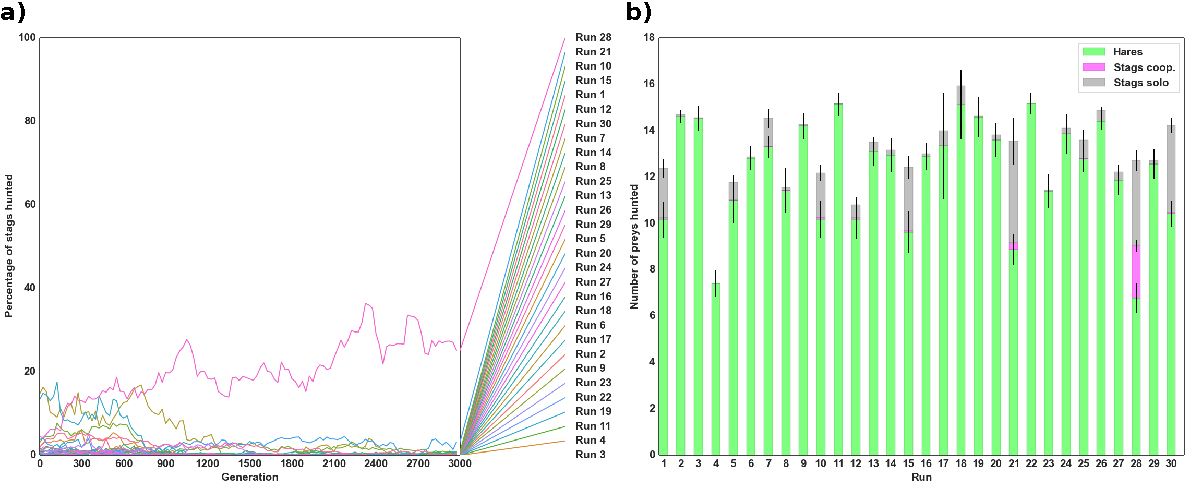
\includegraphics[width=0.5\linewidth]{fig/ArticleBio2/Fig3.png}
        \caption{\textbf{Display of a turning stategy after an entire simulation.}
        Both individuals adopt a \emph{turning} strategy during a complete simulation. The path of the agents is represented in red and blue, starting from their initial positions (represented by black dots). Each disc represents a prey in the environment. Boars are represented in green and stags in purple. When a prey was killed cooperatively, a red cross (resp. blue) is shown on the prey if the red agent (resp. blue) arrived on this prey first.}
      \label{fig:figTurningBehaviour}
    \end{figure}


  \subsection{A more efficient coordination strategy increases the probability to switch to stag hunting}
    In a next experiment, we want to study if the evolution of a different coordination strategy could change the outcome of evolution. More precisely, we are interested in the impact of evolving a less symmetrical strategy. Namely we want the individuals to specialize and adopt different roles. To that end, an individual may now duplicate its neural network and thus co-evolve two networks as its controller (see \emph{Materials and Methods} for more precise explanations). The network adopted as controller during the simulation is randomly selected.

    We show in Figure~\ref{fig:figRecyclingLeadership} a comparison of the number of replicates (out of $30$ in each setting) where the best individual evolved a cooperative strategy on the stags in different settings. The \emph{Control} and \emph{Coordination} settings are defined as in the previous Section and serve as comparison. In the \emph{Coordination+Duplication} setting, the environment is constituted of $18$ prey as in the \emph{Coordination} setting but the duplication of neural networks is possible. We observe that when increasing neural complexity, the transition to the optimum is facilitated as it evolves in $24$ replicates out of $30$. More importantly, the proportion of replicates where the switch to stag hunting occured is significantly higher than without duplication. 

    \begin{figure}[h]
      \centering
        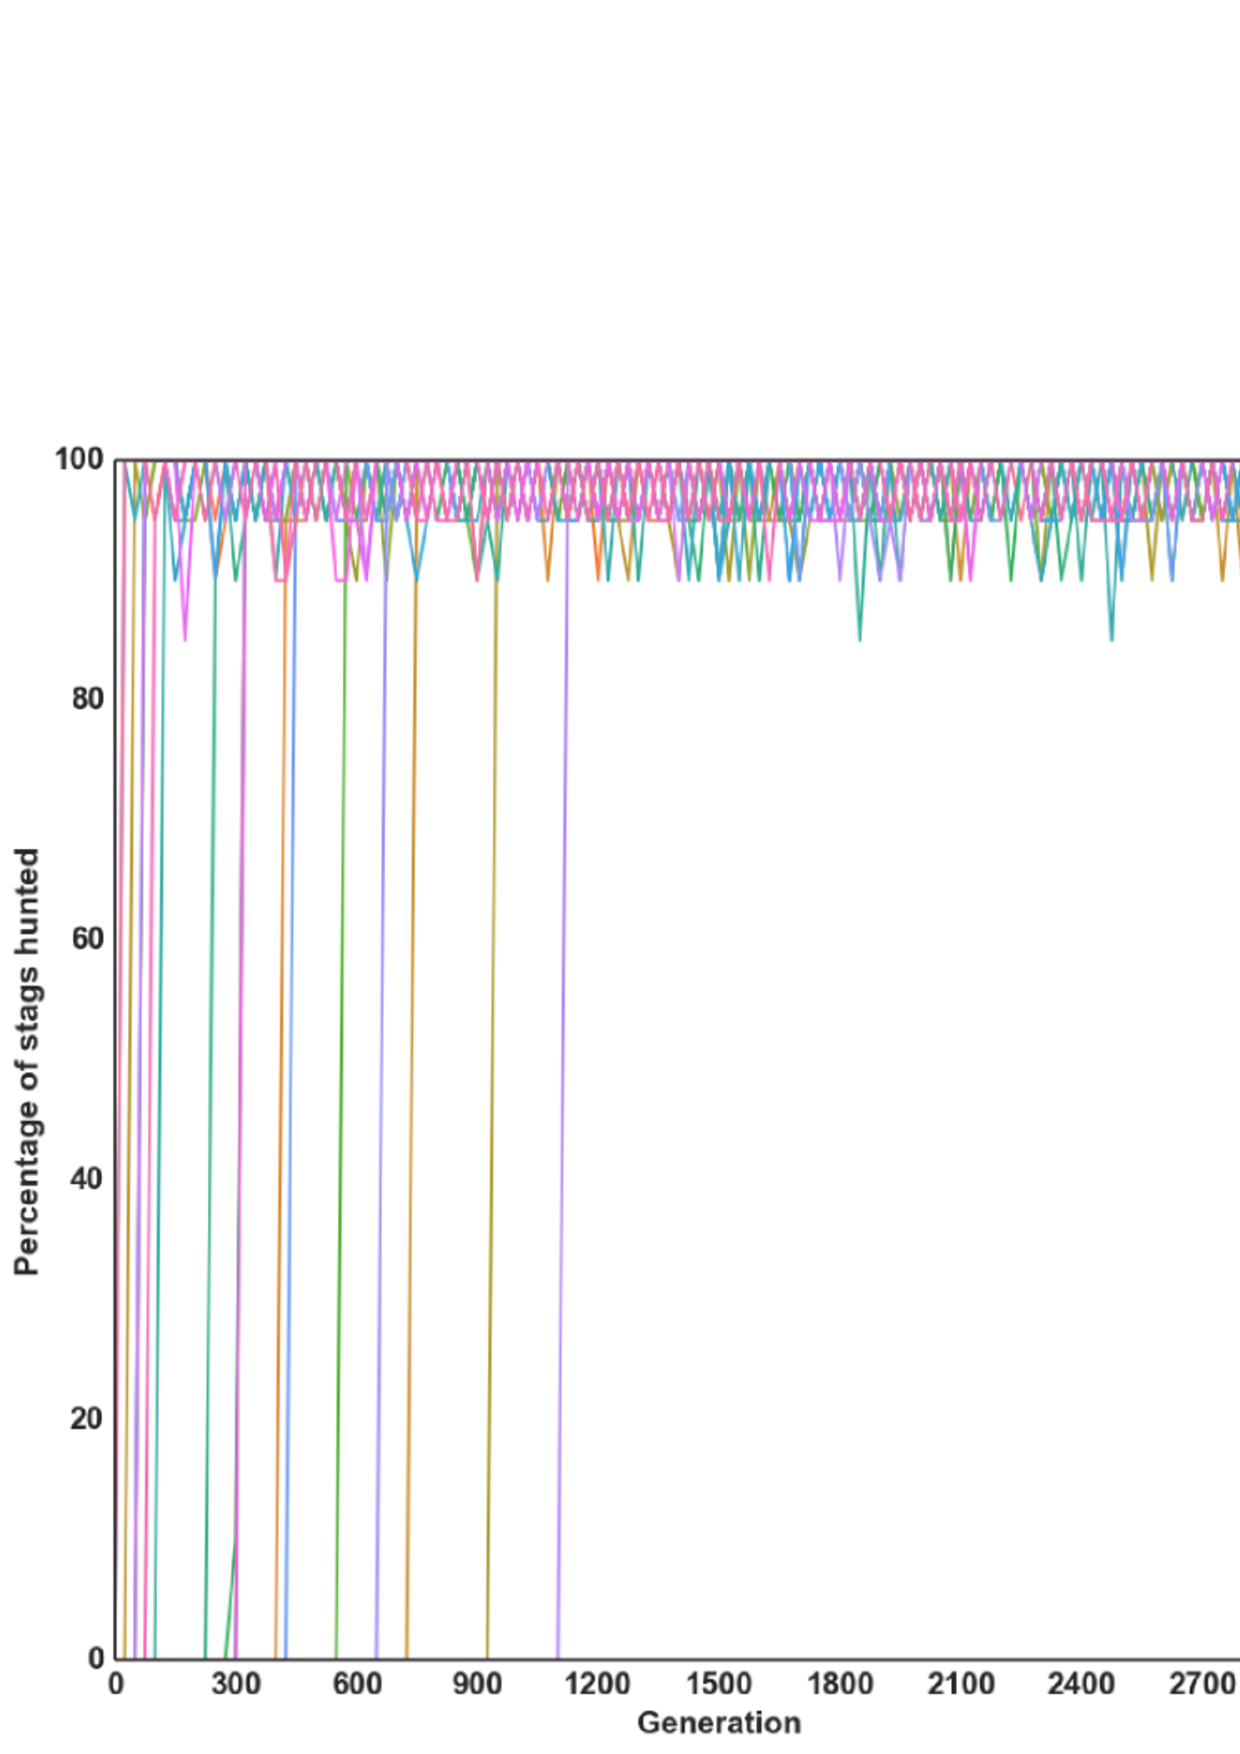
\includegraphics[width=0.7\linewidth]{fig/ArticleBio2/Fig4.png}
        \caption{\textbf{Proportion of cooperative runs.}
        Number of replications (out of a total of $30$) where stag hunting evolved in the \emph{Control}, \emph{Coordination} and \emph{Coordination+Duplication} settings. We consider that stag hunting evolved when more than $50\%$ of the prey hunted were stags hunted cooperatively. In the Control setting, the environment is constituted of one boar and one stag. In comparison, in the Coordination setting, $18$ prey are present in th environment and it is thus necessary to coordinate for cooperation to happen. Finally, in the Coordination+Duplication setting, the environment is also constituted of $18$ prey but individuals have added neural plasticity which allows them to adopt more complex strategies and in particular a leader/follower strategy. Rewards for a boar are 50 if hunted alone and 125 if hunted cooperatively. A stag hunted alone rewards 0 and 250 if hunted in a cooperative fashion (Table~\ref{table:tableRewards}). The population for each of the replications was previously evolved in an environment where hunting stags rewards nothing.}
      \label{fig:figRecyclingLeadership}
    \end{figure}

    There is a drastic difference between the behaviours evolved with and without two networks. Whereas without the duplication of neural networks we revealed that the individuals adopted a turning behaviour, a \emph{leader/follower} strategy was systematically evolved when duplication happened~\ref{fig:figLeadershipBehaviour}. When agents adopt this strategy, they divide between two very different roles. The \emph{leader} looks for prey, gets on them first and checks but rarely on its partner. In comparison, the \emph{follower} tries to keep the leader in its line of sight at all time and join its partner on a common prey. Therefore, in comparison to the coordination strategy previously presented, the individuals adopt asymmetrical behaviours. 

    This second strategy is more efficient than the turning strategy w.r.t. rewards obtained (as shown in Figure~\ref{fig:fitnessRecyclingLeadership}, Mann-Whitney U test on the mean reward at last generation, {\em p}-value \textless 0.001). This can be explained by two main factors. Firstly the hunters are faster, as the decision about which prey to hunt is made by only one of the two individuals. Thus they hunt a significantly higher number of prey. Secondly, the asymmetry in the decision making process implies that they are more precise at hunting. Therefore, the proportion of successful cooperative hunts is significantly greater. Consequently, the leader/follower strategy is a collective behaviour that is both more efficient at hunting cooperatively but also leads to a higher probability to evolve stag hunting.

    \begin{figure}[h]
      \centering
        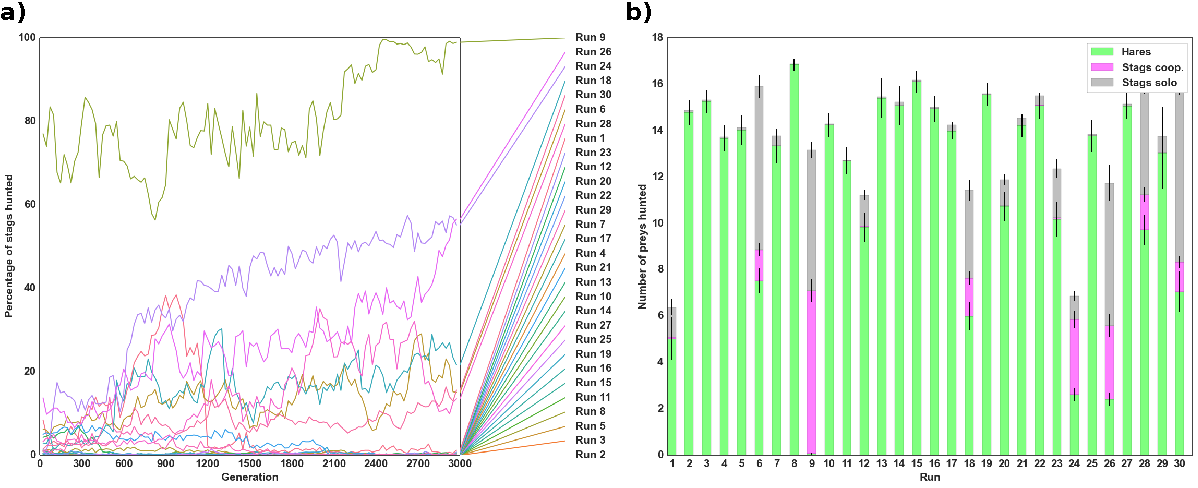
\includegraphics[width=0.5\linewidth]{fig/ArticleBio2/Fig5.png}
        \caption{\textbf{Display of a leader/follower stategy after an entire simulation.}
        Both individuals adopt a leader/follower strategy during a complete simulation. The path of the agents is represented in red and blue, starting from their initial positions (represented by black dots). Each disc represents a prey in the environment. Boars are represented in blue and stags in purple. When a prey was killed cooperatively, a red cross (resp. blue) is shown on the prey if the red agent (resp. blue) arrived on this prey first.}
      \label{fig:figLeadershipBehaviour}
    \end{figure}

    \begin{figure}[h]
      \centering
        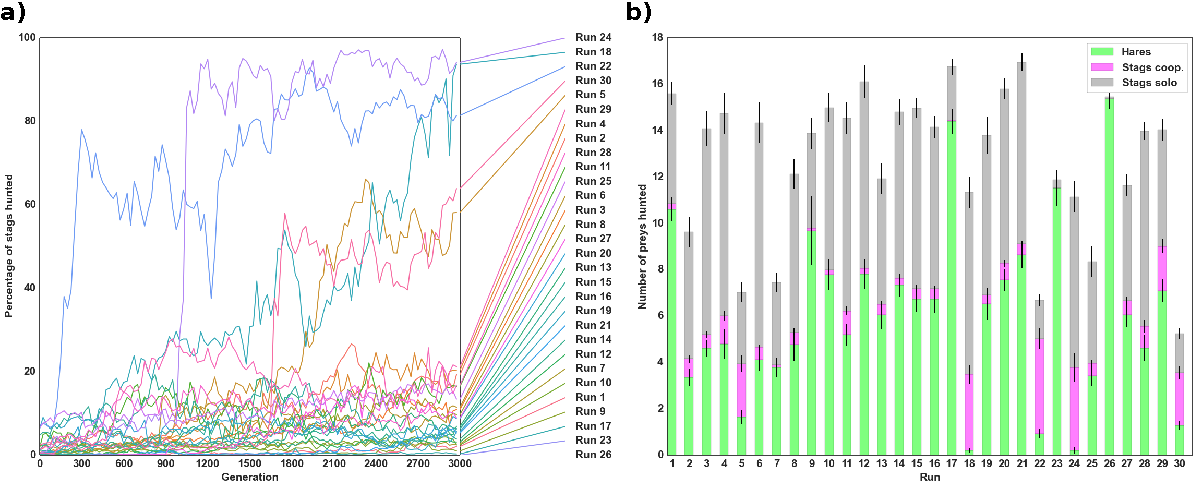
\includegraphics[width=0.7\linewidth]{fig/ArticleBio2/Fig6.png}
        \caption{\textbf{Mean reward comparison of turning and leader/follower strategies.}
        Mean reward of the best individuals in the $30$ replications over evolutionary time by individuals adopting a turning strategy (evolved in the \emph{Coordination} setting) or a leader/follower strategy (evolved in the \emph{Coordination+Duplication} strategy) during the pre-evolution step. Rewards were 50 for a boar if hunted alone, 125 if hunted cooperatively, 0 for a stag hunted alone and 250 if hunted in a cooperative fashion (Table~\ref{table:tableRewards}).}
      \label{fig:fitnessRecyclingLeadership}
    \end{figure}


  \subsection{Similar results are observed when roles are not set}
    We previously showed that the evolution of a leader/follower strategy leads to the more frequent selection of the optimum than with a less efficient strategy. We claim that our results are caused by the general asymmetry in the leader/follower behaviour. Indeed this implies that only one of the two individuals is responsible for the decision making. More precisely, the fact that the two individuals are able to use some asymmetrical cue (i.e. the difference in their neural network) allowed them do decide more efficiently. However, as a hunter chooses which network to use at the start of the simulation, this implies that the individuals keep the same role during a whole evaluation.  We want to study how removing this constraint would impact the results. To that end, we conducted another experiment where both individuals now begin the simulation with the same neural network. They switch to their second neural network only on a specific event during the simulation. In particular, when one of the hunters gets on a prey, the second hunter switches to its second neural network if possible. This is akin to the first hunter signaling that it found a prey to the latter. When the prey is killed, both hunters switch back to their first neural network.

    As in the previous experiment, we compare a \emph{Control} and \emph{Coordination} setting with the \emph{Coordination+Duplication} setting. Only this time, the choice between which neural network to use is done as previously explained. Results are shown in Figure~\ref{fig:figRecyclingComNN}. We see again that the transition to the equilibrium is highly facilitated in the \emph{Coordination+Duplication} setting as in $23$ out of $30$ replicates, there was a transition to the optimal equilibrium. Interestingly, the number of replicates where the transition happened is similar to that of the previous experiment. And again, the number of replicates where optimization occurred is significantly higher with increase neural complexity than without.

    \begin{figure}[h]
      \centering
        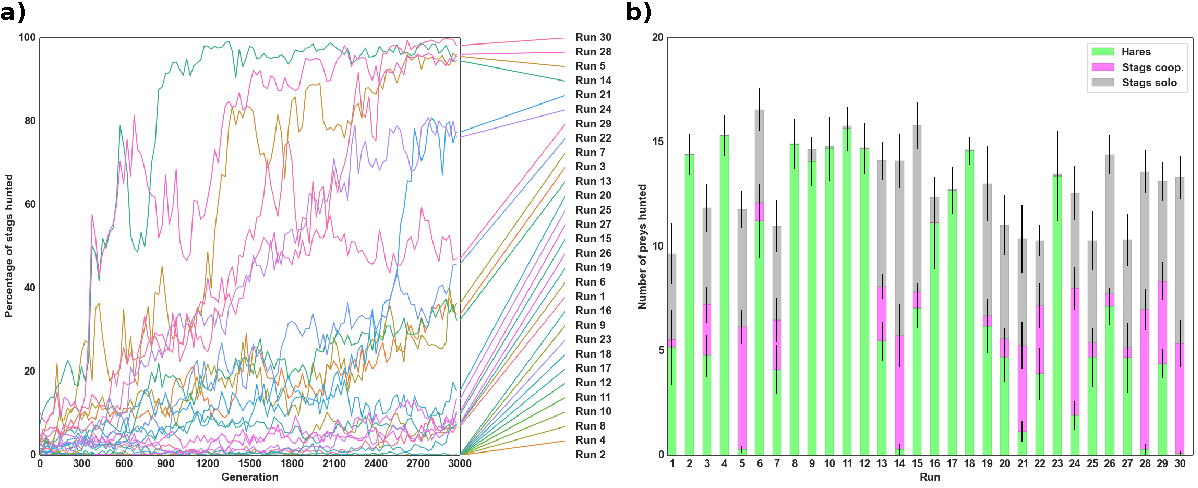
\includegraphics[width=0.7\linewidth]{fig/ArticleBio2/Fig7.png}
        \caption{\textbf{Proportion of cooperative runs.}
        Number of replications (out of a total of $30$) where stag hunting evolved in the \emph{Control}, \emph{Coordination} and \emph{Coordination+Duplication} settings. We consider that stag hunting evolved when more than $50\%$ of the prey hunted were stags hunted cooperatively. In the Control setting, the environment is constituted of one boar and one stag. In comparison, in the Coordination setting, $18$ prey are present in the environment and it is thus necessary to coordinate for cooperation to happen. Finally, in the Coordination+Duplication setting, the environment is also constituted of $18$ prey but individuals have added neural plasticity which allows them to adopt more complex strategies. At a beginning of a simulation, both individuals use the same neural network. A change of network occurs for an individual when the other individual gets on a prey. Rewards for a boar are 50 if hunted alone and 125 if hunted cooperatively. A stag hunted alone rewards 0 and 250 if hunted in a cooperative fashion (Table~\ref{table:tableRewards}). The population for each of the replications was previously evolved in an environment where hunting stags rewards nothing.}
      \label{fig:figRecyclingComNN}
    \end{figure}

    If we look at the behaviours evolved we see the evolution of another similar asymmetrical behaviour, which we call the \emph{search/join strategy}. More precisely, as long as both individuals use the same neural network, they each look for a prey. However, as soon as one of them finds a prey, the switch in networks for the second individual leads to the adoption of a very different behaviour. Even if the collective behaviour is somewhat different from what could be observed in a leader/follower strategy, this strategy is still more efficient than in the turning strategy (Figure~\ref{fig:fitnessRecyclingComNN}, Mann-Whitney U test on the mean reward at last generation, {\em p}-value \textless 0.001).

    \begin{figure}[h]
      \centering
        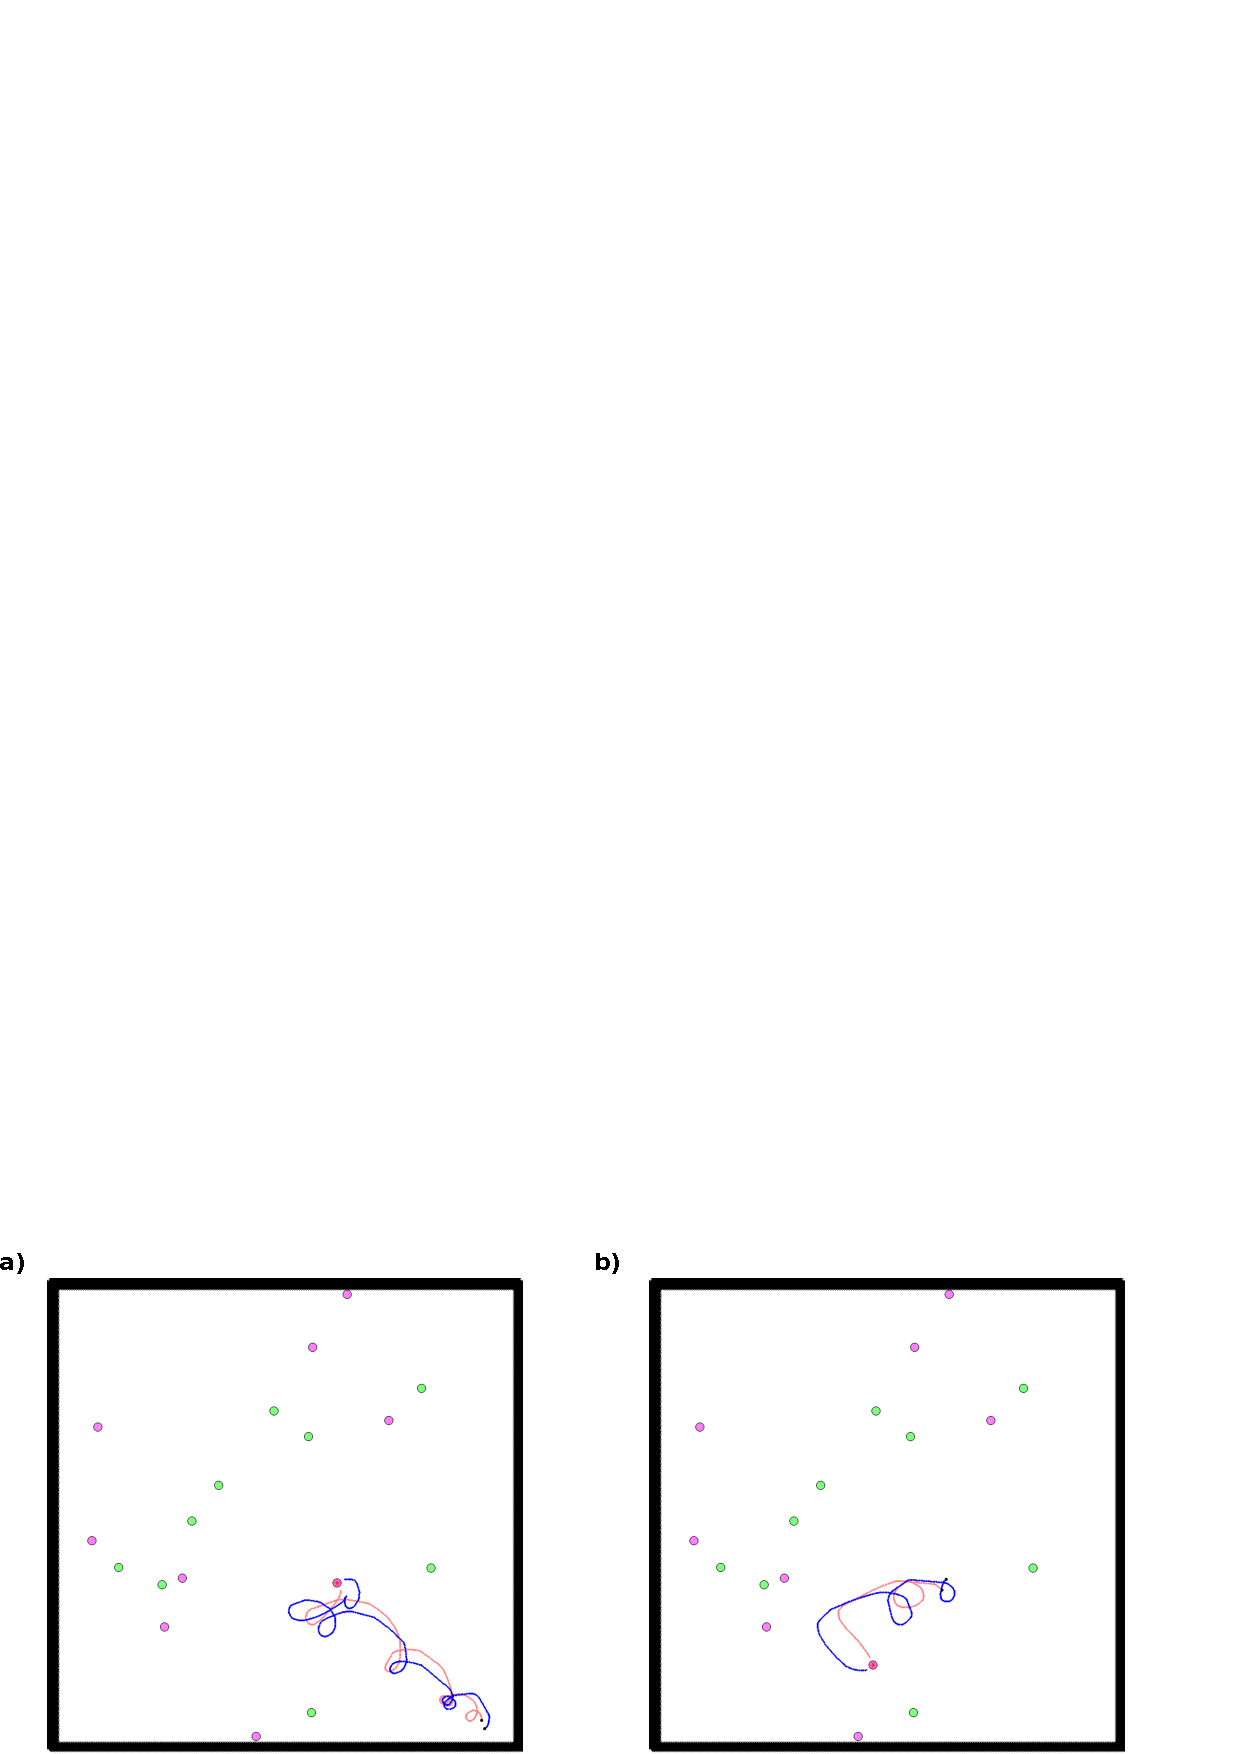
\includegraphics[width=0.7\linewidth]{fig/ArticleBio2/Fig8.png}
        \caption{\textbf{Mean reward comparison of turning and search/join strategies.}
        Mean reward of the best individuals in the $30$ replications over evolutionary time by individuals adopting a turning strategy (evolved in the \emph{Coordination} setting) or a search/join strategy (evolved in the \emph{Coordination+Ducpliation} strategy) during the pre-evolution step. Rewards were 50 for a boar if hunted alone, 125 if hunted cooperatively, 0 for a stag hunted alone and 250 if hunted in a cooperative fashion (Table~\ref{table:tableRewards}).}
      \label{fig:fitnessRecyclingComNN}
    \end{figure} 


  \section{Discussion}
    Because collective hunting is dependent on the simultaneous actions of several individuals, its optimization is difficult. In particular, when a suboptimal equilibrium already evolved, it is not well understood how the group could switch to the optimum through individual adaptation. Here we showed how the nature of coordination strategies could influence this transition. In particular, our simulations in evolutionary robotics revealed that the recycling of a previously evolved coordination strategy could facilite the transition to the optimum. In a simple environment where it was not necessary to coordinate for cooperation to happen, the switch to the optimal equilibrium was impossible. Surprisingly, when the environment is more complex and hunting cooperatively is thus more challenging, we revealed that the transition to the optimum was possible. In particular, when coordination was needed to cooperate, the transition to stag hunting was enabled in a significant number of simulations ($8$ out of $30$). Indeed, the emergence of stag hunting implies that both individuals change their hunting preference. When individuals coordinate, each one react to the behaviour of the other. This means that a change in the hunting preference of one of the two individuals may sometimes lead to both of them hunting stags.

    But the nature of the coordination strategy evolved is also of utmost importance. To highlight this point, we increased the complexity of the neural networks controlling the agents. This was done by allowing the random duplication of neural networks during evolution. We then showed that, depending on the way the choice of network is done, the individuals would evolve two different strategies: a \emph{leader/follower} strategy and a \emph{search/join} strategy. In both of these strategies, the individuals adopt asymmetrical behaviours. We show that when one of these two strategies is evolved, the probability for the transition to the optimal equilibrium to happen is significantly higher (respectively $24$ and $23$ replicates out of $30$). This drastic difference can be explained by the asymmetry of both these behaviours. More precisely, the decision making process of choosing the prey on which to cooperate is now one-sided. In the leader/follower strategy, only the leader chooses the prey. In comparison, in the search/join strategy, as soon as one of the two individuals gets on a prey, the other tries immediatly to join it. This means that, in both cases, the hunting preference of the follower (whether its role is temporary or not) does not matter. In comparison to the previous experiment now the follower only reacts to the leader. This implies that a change in the leader behaviour indirectly changes that of the follower. Consequently, a modification in the hunting preference of the individual choosing the prey is sufficient for cooperation on the stag to occur. The mutational distance is thus decreased by both the recycling \emph{and} the evolution of an asymmetrical coordination strategy. From this, it stems that the probability to switch to stag hunting is higher. 

    More generally, what we reveal through these results is something more critical about the optimization of collective traits. Thanks to the asymmetry of both of these strategies, coordination switched from a collective decision making problem to an individual decision making problem. Initially, the transition to the optimum is a collective problem. Thanks to the asymmetry in the coordination strategy, it now depends on the mutations of a single individual. Furthermore, both of the two strategies are more efficient than the turning strategy which means they can evolve because they are beneficial to the individuals: they are \emph{individually} adaptive. In consequence, individual selection could lead to the adaptation of a collective trait. This suggests that the emergence of other group behaviours may also be explained by such mechanisms, opening a wide range of interesting perspectives on this matter.

